\documentclass{article}
\usepackage[utf8]{inputenc}
\usepackage{amsmath}
\usepackage{enumitem}
\usepackage{esint}
\usepackage{amsthm, amssymb}
\usepackage{graphicx}
\setlength{\jot}{10pt} % affecting the line spacing in the environment
\title{ASTR5420 Problem Set 1}
\author{B. Connor McClellan}
\date{February 2021}

\begin{document}

\maketitle


\section{}
If incident radiation is unpolarized, the differential electron scattering cross section is
%
\begin{equation}
    \frac{d\sigma}{d\Omega} = \frac{3 \sigma_T}{16\pi}(1 + \cos^2 \Theta)
\end{equation}
%
Let the incident photon enter aligned with $\theta=0$ such that the scattering angle $\Theta$ is equal to the colatitude $\theta$.  Integrating over solid angle, we obtain
%
\begin{equation*} \label{exsec}
    \begin{split}
        d\sigma &= \frac{3 \sigma_T}{16\pi}(1 + \cos^2 \theta) d\Omega\\
        %
        \int d\sigma &= \int \frac{3 \sigma_T}{16\pi}(1 + \cos^2 \theta)\ d\Omega \\
        %
        \int_0^\sigma d\sigma &= \int_0^{2\pi}d\phi\int_0^\pi \frac{3 \sigma_T}{16\pi}(1 + \cos^2 \theta)\sin \theta d\theta \\
        %
        \int_0^\sigma d\sigma &= \int_0^{2\pi}d\phi\int_0^\pi \frac{3 \sigma_T}{16\pi}(1 + \cos^2 \theta)\sin \theta d\theta \\
        %
        \sigma &= \frac{3 \sigma_T}{8} \left( -\cos \theta \bigg\rvert_0^\pi - \frac{1}{3}\cos^3 \theta \sin \theta \bigg\rvert_0^\pi\right)\\
        %
        \sigma &= \frac{3 \sigma_T}{8} \left(2 + \frac{2}{3}\right)\\
        %
        \sigma &= \sigma_T \qed
    \end{split}
\end{equation*}
%
The momentum imparted to the electron is determined by the vector difference of the incoming and outgoing photon, which can separated into components assuming the incoming photon lies along the $\hat{z}$ axis.
%
\begin{equation}
    \Delta \mathbf{p} = \frac{h\nu'}{c} \mathbf{\hat n'} - \frac{h\nu}{c}\mathbf{\hat n}
\end{equation}
%
As we have established, the incoming photon direction $\mathbf{\hat n}$ is equal to $\hat{z}$ while the outgoing photon direction is 
%
\begin{equation}
    \mathbf{\hat n'} = \sin \theta \cos{\phi}\ \hat{x} + \sin \theta \sin \phi\ \hat{y}  + \cos \theta \ \hat{z}
\end{equation}
%
Since we assume the energy of the photon is unchanged during the scattering, $\nu' = \nu$. Then the vector difference yields

\begin{equation}
    \Delta \mathbf{p} = \frac{h\nu}{c}\sin \theta \cos \phi\ \hat{x} + \frac{h\nu}{c}\sin \theta \sin \phi\ \hat{y} + \frac{h\nu}{c}\left(\cos \theta - 1\right)\ \hat{z}
\end{equation}
%
Converting to spherical coordinates to get the radial component of this vector, we obtain
\begin{equation}
    \boxed{\Delta \mathbf{p} = \frac{h\nu}{c}\left(1-\cos\theta\right)\ \hat{r}}
\end{equation}
As expected, this has the right limits: when the scattering angle is $\pi$, the photon bounces right back in the direction it came and the imparted momentum is $2h\nu/c$. If the scattering angle is $0$, the photon continues along its trajectory unchanged and no momentum is imparted. 

We now wish to find the radiation force per electron in the radial direction. The spectral energy $dL/d\nu$ can be converted to units of photons per unit time per unit area per frequency by dividing through by the energy per photon, which is $h\nu$, and the surface area of the sphere. Then, multiplying by the momentum imparted to the electron by the scattering, we obtain a momentum per unit time per unit area per frequency. Finally, the differential cross section introduces units of area and solid angle which integrate out to a force.
%
\begin{equation}
    \begin{split}
    \frac{df_{\mathrm{rad}}}{d\nu d\Omega} = \frac{\left(\frac{dL}{d\nu}\right)}{4\pi r^2 h\nu}\times \frac{h\nu}{c}\left(1 - \cos \theta \right) \times \frac{d\sigma}{d\Omega} \\
    %
    \end{split}
\end{equation}
%
Integrating over frequency and solid angle $d\Omega = \sin \theta \ d\theta\ d\phi$, we obtain

\begin{equation*}
    \begin{split}
    f_{\mathrm{rad}} &= \int
\int\frac{1}{4\pi r^2}\frac{dL}{d\nu}\times \frac{1}{c}\left(1 - \cos \theta \right) \times \frac{3 \sigma_T}{16\pi}(1 + \cos^2 \theta) d\Omega d\nu\\
%
&= \frac{3 \sigma_T L}{32\pi r^2 c} \int_0^\pi \left(1 - \cos \theta \right)(1 + \cos^2 \theta) \sin \theta d\theta\\
&= \frac{3 \sigma_T L}{32\pi r^2 c} \left(\frac{8}{3}\right)\\
&= \frac{\sigma_T L}{4\pi r^2 c} \qed
    \end{split}
\end{equation*}

\section{}

\begin{enumerate}[label=\alph*.]
\item
\begin{equation*}
    \begin{split}
        \vec{f}_{\mathrm{rad}} &= -\vec{f}_{\mathrm{grav}}\\
        %
        \frac{\sigma_T \vec{F}}{c} &= m_p \nabla \phi\\
        %
        \frac{\sigma_T}{c}\vec{F}\cdot \hat{n} &= m_p \nabla \phi \cdot \hat{n}\\
        %
        \frac{\sigma_T}{c} \oiint_S \vec{F}\cdot \hat{n} \ dS &= m_p \oiint_S \nabla \phi \cdot \hat{n} \ dS\\
        %
    \end{split}
\end{equation*}
\begin{equation}
    \boxed{\frac{\sigma_T L}{c} = m_p \oiint_S \nabla \phi \cdot \hat{n} \ dS\\}
\end{equation}
%
\item
\begin{equation*}
    \begin{split}
        \frac{\sigma_T L}{c} = m_p \oiint_S \nabla \phi \cdot \hat{n} \ dS\\
        \frac{\sigma_T L}{c} = m_p \iiint_V \nabla \cdot \nabla \phi \ dV\\
    \end{split}
\end{equation*}
We now recognize the Poisson equation for Newtonian gravity is $\nabla \cdot \nabla \phi = \nabla^2\phi = 4\pi G\rho$ and make the necessary substitution.
\begin{equation*}
    \begin{split}
        \frac{\sigma_T L}{c} &= 4\pi G m_p \iiint_V \rho \ dV\\
    \end{split}
\end{equation*}
\begin{equation}
    \boxed{\frac{\sigma_T L}{c} = 4\pi G m_p M_{\mathrm{enc}}}
\end{equation}
%
\item
Solving for L, we obtain
\begin{equation}
    \boxed{L = \frac{4\pi G M_{\mathrm{enc}} m_p c}{\sigma_T}}
\end{equation}
This differs from the spherical result only by the fact that $M$ is the mass enclosed by the volume $V$, which is not necessarily spherically symmetric.
\end{enumerate}

\section{}

\begin{figure}
    \centering
    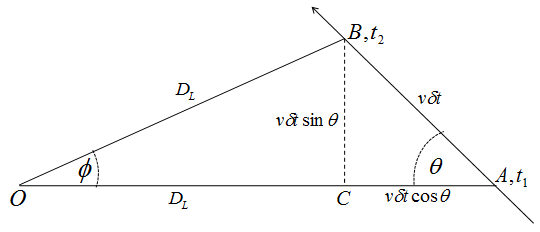
\includegraphics[width=
\textwidth]{Superluminal_motion_in_AGN_jets.png}
    \caption{Superluminal motion diagram}
    \label{fig:my_label}
\end{figure}

\begin{enumerate}[label=\alph*.]
    \item Using the diagram in Fig. \ref{fig:my_label}, we begin by examining the two events A and B in the frame of the observer, O. The time interval $\delta t$ is equal to $t_2 - t_1$, while the events seen by the observer are
    
    \begin{equation}
        t_2' = t_2 + \frac{D}{c}
    \end{equation}
    \begin{equation}
        t_1' = t_1 + \frac{D + v\delta t \cos \theta}{c}
    \end{equation}
    And thus, the time interval seen by the observer is
    \begin{equation}
        \begin{split}
            \delta t' = t_2' - t_1' &= t_2 + \frac{D}{c} - t_1 - \frac{D + v\delta t \cos \theta}{c}\\
            &=  \delta t - \frac{v\delta t \cos \theta}{c}\\
        \end{split}
    \end{equation}
    The apparent velocity is defined as 
    \begin{equation}
        v_{\textrm{app}} = \frac{D\phi}{\delta t'}
    \end{equation}
    Since the angle $\phi$ is small, we utilize the approximation $\phi \approx \sin \phi$ to obtain
    \begin{equation}
        v_{\textrm{app}} = \frac{D\sin \phi}{\delta t'} = \frac{v \delta t \sin \theta}{\delta t - \frac{v}{c}\delta t \cos \theta} = \frac{v\sin \theta}{1 - \frac{v}{c} \cos \theta} \qed
    \end{equation}
    \item To find the maximum,  we take the derivative of $v_{\textrm{app}}$ with respect to $\theta$ and set it to zero. Then, we solve for the angle. 
    \begin{equation}
        \begin{split}
            \frac{dv_{\textrm{app}}}{d\theta} &= \frac{d}{d\theta} \frac{v\sin \theta}{1 - \frac{v}{c} \cos \theta} = 0\\
            0 &= \frac{v\cos\theta}{1 - \frac{v}{c}\cos \theta} - \frac{v\sin\theta}{\left(1 - \frac{v}{c}\cos\theta\right)^2}\left(\frac{v}{c}\sin\theta\right)\\
            & = \cos\theta -\frac{v}{c}\cos^2\theta  - \frac{v}{c}\sin^2\theta
        \end{split}
    \end{equation}
    \begin{equation}
        \boxed{\theta_\textrm{max} = \cos^{-1} \left(\frac{v}{c}\right)}
    \end{equation}
    We now plug this in to the expression for $v_\textrm{app}$ to find the maximum apparent velocity in terms of $v$ and $\gamma$.
    \begin{equation}
        \begin{split}
            v_{\textrm{max}} &= \frac{v\sin \left[\cos^{-1} \left(\frac{v}{c}\right)\right]}{1 - \frac{v}{c} \cos \left[\cos^{-1} \left(\frac{v}{c}\right)\right]}\\
            &= \frac{v\sqrt{1 - \frac{v^2}{c^2}}}{1 - \frac{v^2}{c^2}} \\
            & = v \gamma
        \end{split}
    \end{equation}
\end{enumerate}

\end{document}
